\section{Kerberos Authentication}
\label{windows:authentication:kerberos}

\subsection{major Components}

The Kerberos protocol defines how  clients interact with a network authentication service. Clients obtain  tickets from the Kerberos Key Distribution Center (KDC), and they submit  these tickets to application servers when connections are established.  It uses UDP port 88 by default and depends on the process of symmetric  key cryptography.
“Kerberos uses tickets to authenticate a user and completely avoids sending passwords across the network”.
There are some key components in Kerberos authentication that play a crucial role in the entire authentication process.
\begin{figure}
  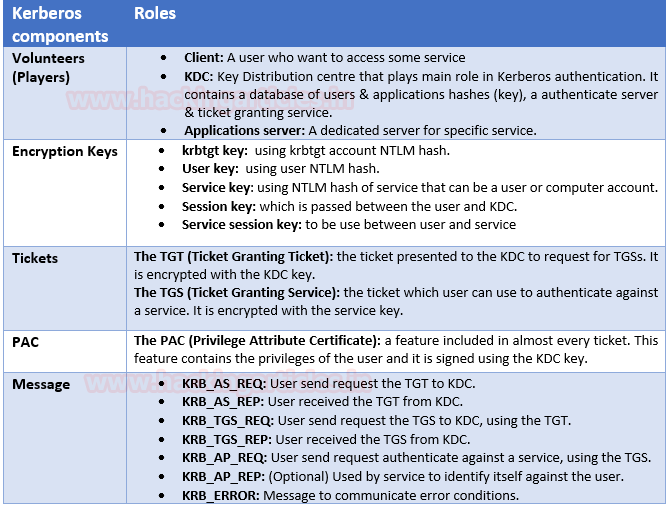
\includegraphics[width=\linewidth]{windows_knowledge/authentication/images/kerb-components.png}
  \caption{Kerberos components}
  \label{fig:kerberos-components}
\end{figure}

\subsection{workflow}

In the Active Directory domain, every  domain controller runs a KDC (Kerberos Distribution Center) service that  processes all requests for tickets to Kerberos. For Kerberos tickets,  AD uses the KRBTGT account in the AD domain.
The image below shows that the major  role played by KDC in establishing a
secure connection between the  server \& client and the entire process uses some special components  as defined in the table above.

\begin{figure}
  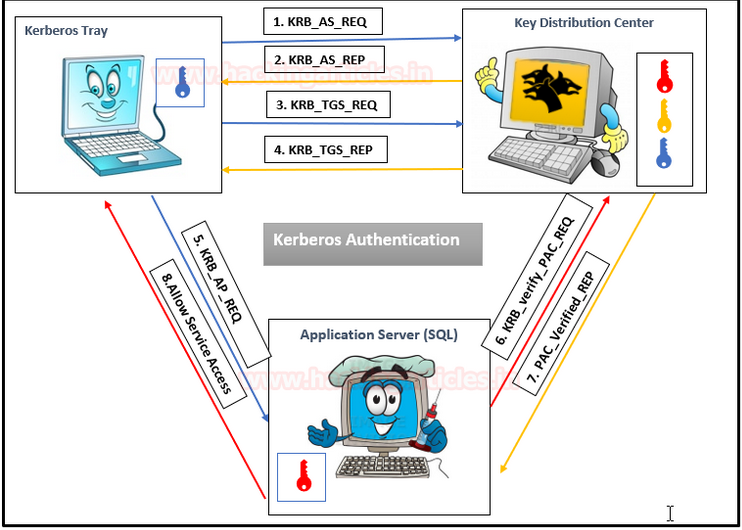
\includegraphics[width=\linewidth]{windows_knowledge/authentication/images/kerb-all.png}
  \caption{Kerberos Workflow}
  \label{fig:kerberos-workflow}
\end{figure}


As mentioned above, Kerberos uses  symmetric cryptography for encryption and decryption. Let us get into  more details and try to understand how encrypted messages are sent to  each other. Here we use three colours to distinguish Hashes:
\begin{itemize}
    \item \verb+BLUE _KEY+: User NTLM HASH
    \item \verb+YELLOW_KEY+: Krbtgt NTLM HASH
    \item \verb+RED_KEY+: Service NTLM HASH
\end{itemize}

\subsubsection*{Step 1: Communication initialization}
\verb+KRB_AS_REQ+ contains the following:
\begin{itemize}
    \item Username of the client to be authenticated.
    \item The service SPN (SERVICE PRINCIPAL NAME) linked with Krbtgt account
    \item An encrypted timestamp (Locked with User Hash: Blue Key)
\end{itemize}

The entire message is encrypted using the User NTLM hash (Locked with BLUE KEY) to authenticate the user and prevent replay attacks.

\subsubsection*{Step 2}

The KDC uses a database consisting of Users/Krbtgt/Services hashes to decrypt a message (Unlock with BLUE KEY) that authenticates user identification.
Then KDC will generate TGT (Ticket  Granting Ticket) for a client that is
encrypted using Krbtgt hash  (Locked with Yellow Key) \& some Encrypted Message using User Hash.

\verb+KRB_AS_REP+ contains the following:
\begin{itemize}
    \item  Username
    \item  Some encrypted data, (Locked with User Hash: Blue Key) that contains: 
    \begin{itemize}
        \item  Session key
        \item  The expiration date of TGT
    \end{itemize}
    \item  TGT, (Locked with Krbtgt Hash: Yellow Key) which contains:
    \begin{itemize}
        \item  Username
        \item  Session key
        \item  The expiration date of TGT
        \item  \gls{win:PAC}~\ref{windows_knowledge:ad:kerberos:PAC}
 with user privileges, signed by KDC
    \end{itemize}
\end{itemize}

\begin{figure}
  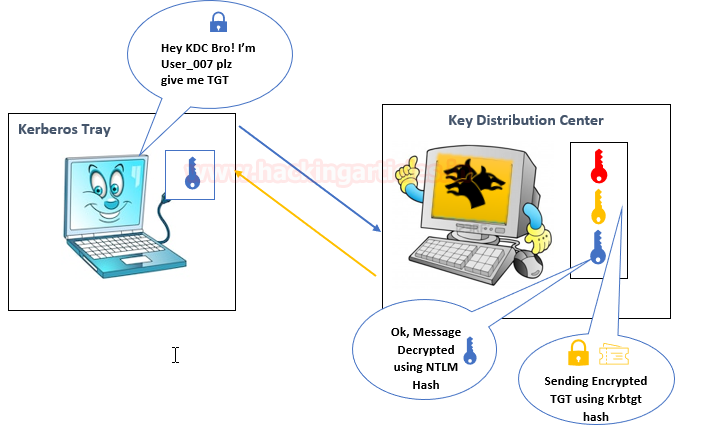
\includegraphics[width=\linewidth]{windows_knowledge/authentication/images/kerb-1.png}
  \caption{Kerberos TGT}
  \label{fig:kerberos-tgt}
\end{figure}

\begin{figure}
  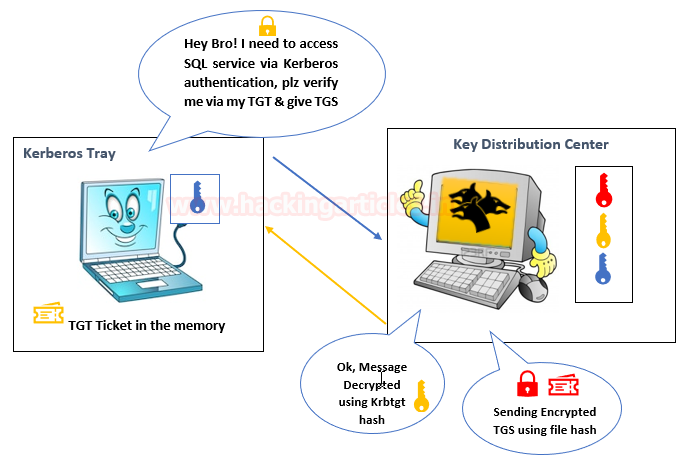
\includegraphics[width=\linewidth]{windows_knowledge/authentication/images/kerb-2.png}
  \caption{Kerberos TGS}
  \label{fig:kerberos-tgs}
\end{figure}

\begin{figure}
  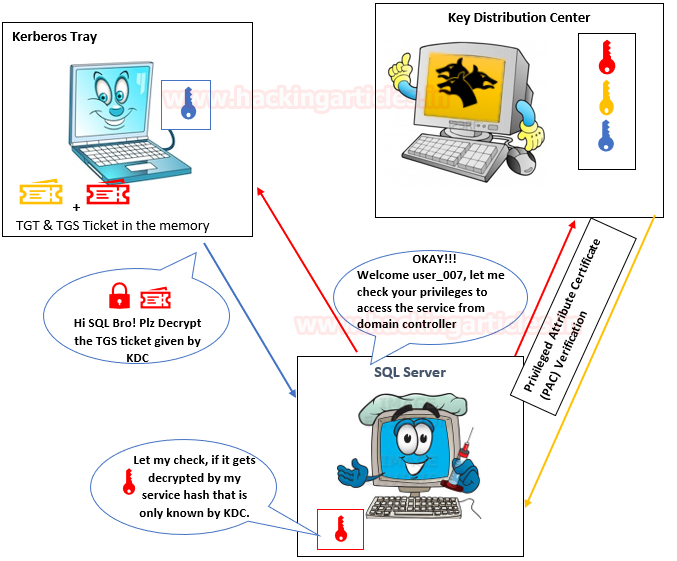
\includegraphics[width=\linewidth]{windows_knowledge/authentication/images/kerb-3.png}
  \caption{Kerberos Service Authentication}
  \label{fig:kerberos-service}
\end{figure}

\subsubsection*{Step 3}
The \verb+KRB_TGT+ will be stored in the Kerberos tray (Memory) of the client
machine, as the user already has the \verb+KRB_TGT+, which is used to identify  himself for the TGS request. The client sent a copy of the TGT with the  encrypted data to KDC.

\verb+KRB_TGS_REQ+ contains:
\begin{itemize}
    \item Encrypted data with the session key
    \begin{itemize}
        \item Username
        \item Timestamp
    \end{itemize}
    \item TGT
    \item SPN of requested service e.g. SQL service
\end{itemize}


\subsubsection*{Step 4}

The KDC receives the \verb+KRB_TGS_REQ+ message and decrypts the message using
Krbtgt hash to verify TGT (Unlock using Yellow key), then KDC returns a  TGS as
\verb+KRB_TGS_REP+ which is encrypted using requested service hash (Locked with
Red Key) and Some Encrypted Message using User Hash.

\verb+KRB_TGS_REP+ contains:
\begin{itemize}
    \item Username
    \item Encrypted data with the session key:
    \begin{itemize}
        \item Service session key
    \end{itemize}
    \item The expiration date of TGS
    \item TGS, (Service Hash: RED Key) which contains:
    \begin{itemize}
        \item  Service session key
        \item Username
        \item The expiration date of TGS
        \item  \gls{win:PAC}~\ref{windows_knowledge:ad:kerberos:PAC}
 with user privileges, signed by KDC
    \end{itemize}
\end{itemize}


\subsubsection*{Step 5}
The user sent the copy of TGS to the Application Server,\verb+KRB_AP_REQ+ contains:
\begin{itemize}
    \item TGS
    \item Encrypted data with the service session key:
    \begin{itemize}
        \item Username
        \item Timestamp, to avoid replay attacks
    \end{itemize}
\end{itemize}

\subsubsection*{Step 6}
The  application attempts to decrypt the message using its NTLM hash and to  verify the PAC from KDC to identify user Privilege which is an optional  case.
\subsubsection*{Step 7}
KDC verifies PAC (Optional)
\subsubsection*{Step 8}
Allow the user to access the service for a specific time.

\subsection{\gls{win:PAC}}
\label{windows_knowledge:ad:kerberos:PAC}
PAC is double encrypted (SPN hash) signed by the KDC hash.

Critical services in term of perf (MSSQL) don't ask the KDC to verify this open to PAC forgery attack

\url{https://stealthbits.com/blog/what-is-the-kerberos-pac/}


\subsection{Service Principal Name (SPN)}
\label{windows_knowledge:ad:kerberos:SPN}
\index{Active Directory!SPN}

\gls{win:SPN}s are unique identifiers that Kerberos uses to map a service
instance to a service account in whose context the service is running. Domain
accounts are often used to run services to overcome the network authentication
limitations of built-in accounts such as \verb+NT AUTHORITY\LOCAL SERVICE+

Active Directory Domain  Services and Windows provide support for Service Principal Names (SPNs),  which are key components of the Kerberos mechanism through which a  client authenticates a service.

Domain accounts running services are often local administrators, if not highly
privileged domain accounts. Due to the distributed nature of systems,
interacting services, and associated data transfers, service accounts may be
granted administrator privileges on multiple servers across the enterprise.
Many services require elevated privileges on various systems, so service
accounts are often added to privileged groups, such as Domain Admins, either
directly or via nested membership. {\bf Finding SPNs associated with highly
privileged accounts in a Windows environment is very common}. 

Important Points:
\begin{enumerate}
\item If you install multiple instances of a service on computers throughout a forest, each instance must have its SPN. 
\item Before the Kerberos authentication service can use an SPN to authenticate a service, the SPN must be registered on the account.
\item A given SPN can be registered on only one account. 
\item An SPN must be unique in the forest in which it is registered.
\item If it is not unique, authentication will fail.
\end{enumerate}

\subsubsection{SPN format}
\verb+<ServiceClass>/<host>:<port> <serviceName>+
\begin{itemize}
    \item \verb+ServiceClass+: \verb+HTTP, LDAP,MSSQLSVC+ \ldots
    \item \verb+host+: \verb+<DomainName>/wMachineName>+
\end{itemize}


\subsubsection{Type of SPN}
\begin{itemize}
\item Host-based SPNs which is associated  with the computer account in AD, it is randomly generated 128-character  long password which is changed every 30 days, hence it is no use in  Kerberoasting attacks
\item SPNs that have been associated with a domain user account where NTLM hash will be used.
\end{itemize}

\subsection{Pre-authentication}
\label{windows:authentication:kerberos:preauthentication}

Pre-authentication requires that requestors prove their identity before the KDC will issue a ticket for a particular principal. There are several types of pre-authentication defined by the Kerberos Clarifications document. However, only the  encrypted timestamp (PA-ENC-TIMESTAMP) pre-authentication method is commonly implemented.

Pre-authentication is controlled by KDC policy. If a user attempts to acquire
initial tickets through the AS exchange, but the KDC requires
pre-authentication, then the KDC will send a \verb+KRB_ERROR+ message instead
of an \verb+AS_REP+ in reply to the client AS request. This \verb+KRB_ERROR+ message tells the client that pre-authentication is required. If the KDC responds with the error \verb+PRINCIPAL UNKNOWN+, the username is invalid.

This request used for username enumeration does not cause logon failures and will not
lock out accounts.



After the enumeration of user accounts is finished, we can attempt to abuse a
feature within Kerberos with an attack method called \verb+ASREPRoasting+. ASReproasting occurs when a user account has the privilege "Does not require Pre-Authentication" set. This means that the account does not need to provide valid identification before requesting a Kerberos Ticket on the specified user account.

The Kerberos protocol defines how  clients interact with a network authentication service. Clients obtain  tickets from the Kerberos Key Distribution Center (KDC), and they submit  these tickets to application servers when connections are established.  It uses UDP port 88 by default and depends on the process of symmetric  key cryptography.
“Kerberos uses tickets to authenticate a user and completely avoids sending passwords across the network”.
There are some key components in Kerberos authentication that play a crucial role in the entire authentication process.

This method does not generate Windows event ID
\href{https://docs.microsoft.com/en-us/windows/security/threat-protection/auditing/event-4625}{4625:
An account failed to log on}, or a logon failure which is often monitored for.

\url{https://ldapwiki.com/wiki/Kerberos%20Pre-Authentication}

\subsection{MIT vs Microsoft}
\url{https://www.techblog.moebius.space/posts/2018-05-25-kerberos-an-overview-of-principals-and-keytabs/#keytabs}

Kerberos uses a key agreement process to exchange messages. Both the  client and KDC know the users "long term credential" which is their  password hashed using a specific key derivation function. When the  client wants to send a message to the KDC, it encrypts it using the long  term credential. The KDC knows that credential so it can decrypt it.  The response is encrypted in the same way.
Neither party sends the password or its hash to the other in general use.


\subsection{Keytabs}
In most cases, end-users would authenticate to the KDC using their  client secret (i.e their password). However, it would be cumbersome for  automated scripts and applications to regularly (re)authenticate using a  password.
This is where it might make sense to use a keytab. A keytab (Key  Table), is a file storing pairs of Kerberos principals and their keys.  When users generally start the authentication process using kinit, they  are prompted for their password - which triggers the KDC to provide it  the TGT, and then initiate the follw-up requests for service tickets.  What the keytab does is when the client wishes to initiate  authentication, the password is sent automatically to the KDC (in  encrypted form) from the keytab file, rather than prompting for it.
The consequences of this are fairly obvious. Anyone who has access to  a keytab can essentially impersonate the principal(s) contained within  it. So its safe to say that keytabs should be protected just like  passwords.

\subsection{Links}
\begin{itemize}
    \item \url{https://www.roguelynn.com/words/explain-like-im-5-kerberos/}
    \item \url{https://www.kerberos.org/software/tutorial.html}
\end{itemize}
